% Le couloir : une case par déplacement
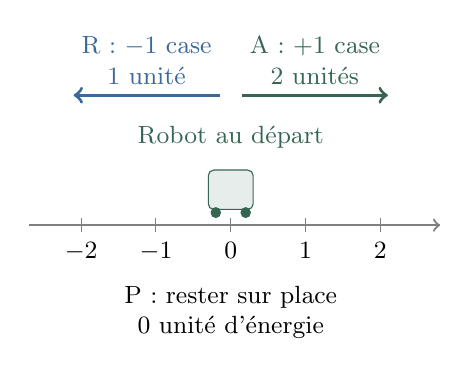
\begin{tikzpicture}[x=0.95cm,y=1cm,font=\small]
\definecolor{vert}{RGB}{53,102,81}
\definecolor{bleu}{RGB}{59,105,153}
\draw[->,gray,thick] (-2.7,0) -- (2.8,0);
\foreach \x in {-2,-1,0,1,2} {
  \draw[gray] (\x,-0.09) -- (\x,0.09);
  \node[below] at (\x,-0.1) {$\x$};
}
\draw[fill=vert!12,draw=vert,rounded corners=2pt] (-0.3,0.2) rectangle (0.3,0.7);
\fill[vert] (-0.2,0.16) circle (0.07);
\fill[vert] (0.2,0.16) circle (0.07);
\node[above,text=vert] at (0,0.85) {Robot au d\'epart};
\draw[->,very thick,vert] (0.15,1.65) -- (2.1,1.65)
  node[midway,above,align=center] {A : $+1$ case\\2 unit\'es};
\draw[->,very thick,bleu] (-0.15,1.65) -- (-2.1,1.65)
  node[midway,above,align=center] {R : $-1$ case\\1 unit\'e};
\node[below,align=center] at (0,-0.65) {P : rester sur place\\0 unit\'e d'\'energie};
\end{tikzpicture}
